../cictikz/src/cictikz/data/tex/cictikz_preamble.tex

% Bluetooth LE advertising, redrawn as a message sequence chart from the
% Nordic Semiconductor DevZone figure: the peripheral transmits an
% advertisement once per advertisement interval, the central opens its
% receiver for a scan window once per scan interval, and when a scan
% catches an advertisement the central may answer with a connection
% request. The three interval annotations are the whole protocol: the
% two sides never agreed on a schedule, they only overlap often enough.

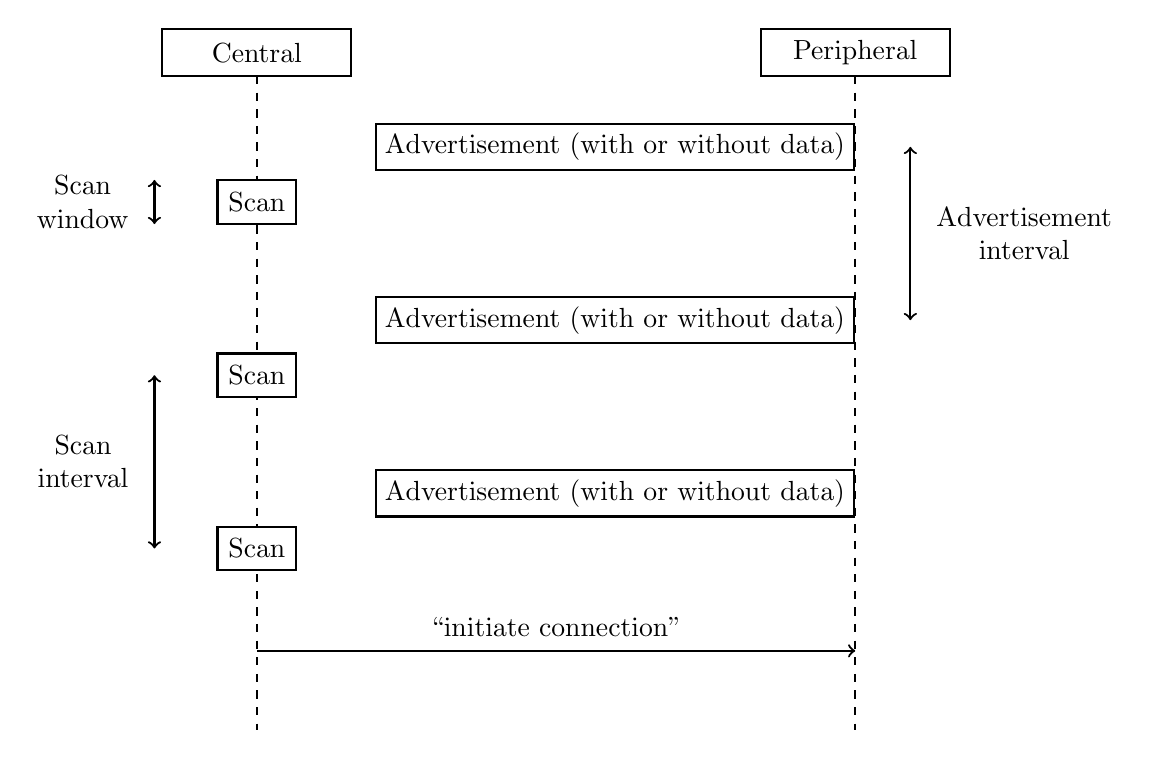
\begin{tikzpicture}[thick]

  \def\xc{0} \def\xp{7.6}

  \node[draw, minimum width=2.4cm, minimum height=0.6cm] (hc) at (\xc,0) {Central};
  \node[draw, minimum width=2.4cm, minimum height=0.6cm] (hp) at (\xp,0) {Peripheral};
  \draw[dashed] (\xc,-0.3) -- (\xc,-8.6);
  \draw[dashed] (\xp,-0.3) -- (\xp,-8.6);

  \foreach \y in {-1.2,-3.4,-5.6} {
    \draw (\xp,\y) node[draw, anchor=east, minimum height=0.55cm, fill=white]
      {Advertisement (with or without data)};
  }
  \foreach \y in {-1.9,-4.1,-6.3} {
    \node[draw, minimum width=1.0cm, minimum height=0.55cm, fill=white]
      at (\xc,\y) {Scan};
  }

  \draw[<->] (-1.3,-1.62) -- (-1.3,-2.18);
  \node[anchor=east, align=center] at (-1.5,-1.9) {Scan\\window};
  \draw[<->] (-1.3,-4.1) -- (-1.3,-6.3);
  \node[anchor=east, align=center] at (-1.5,-5.2) {Scan\\interval};
  \draw[<->] (8.3,-1.2) -- (8.3,-3.4);
  \node[anchor=west, align=center] at (8.5,-2.3) {Advertisement\\interval};

  \draw[->] (\xc,-7.6) -- (\xp,-7.6);
  \node[anchor=south] at (3.8,-7.55) {``initiate connection''};

\end{tikzpicture}
\end{document}
